\subsection{Lower Bound in SMAB}    
    
    SMAB problems have been extensively studied in several earlier works such as \citet{thompson1933likelihood},  \citet{thompson1935theory}, \citet{robbins1952some} and \citet{lai1985asymptotically}. Lai and Robbins in  \citet{lai1985asymptotically} established an asymptotic lower bound for the cumulative regret. It showed that for any consistent allocation strategy, we can have
\begin{align*}
\liminf_{T \to \infty}\frac{\E[R_{T}]}{\log T}\geq\sum_{\{i:r_{i}<r^{*}\}}\frac{(r^{*}-r_{i})}{KL(Q_{i}||Q^{*})}
\end{align*}    
where $KL(Q_{i}||Q^{*})$ is the Kullback-Leibler divergence between the reward densities $Q_{i}$ and $Q^{*}$, corresponding to arms with mean $r_{i}$ and $r^{*}$, respectively.

\subsection{The Upper Confidence Bound Approach}
    
    Over the years SMABs have seen several algorithms with strong regret guarantees. For further reference, an interested reader can look into \citet{bubeck2012regret}. In the next few subsections, we will explicitly focus on the upper confidence bound algorithms which is a type of non-Bayesian algorithm widely used in SMAB setting. The upper confidence bound or UCB algorithms balance the exploration-exploitation dilemma by linking the uncertainty in the estimate of an arm with the number of times an arm is pulled and therefore ensuring sufficient exploration. 
    
\subsubsection{UCB1 Algorithm}    
    
    
    One of the earliest among these algorithms is UCB1 algorithm proposed first in \citet{agrawal1995sample} and subsequently analyzed in \citet{auer2002finite}. The UCB1 algorithm (as stated in \citet{auer2002finite}) is mentioned in Algorithm \ref{alg:ucb1}.
    
\begin{algorithm}[!th]
\caption{UCB1}
\label{alg:ucb1}
\begin{algorithmic}[1]
\State \textbf{Input:} $K$ number of arms with unknown parameters of reward distribution
\State Pull each arm once
 \For{$t=K+1,..., T$}
\State Pull the arm such that $\argmax_{i\in A}\bigg\lbrace\hat{r}_{i} + \sqrt{\dfrac{2\log (t)}{z_i}}\bigg\rbrace$
\State $t:=t+1 $
 \EndFor
\end{algorithmic}
\end{algorithm}
    
    The intuition behind this algorithm is simple and it follows from the ideas of concentration inequalities in probability measure theory. The term $\sqrt{\dfrac{2\log (t)}{z_i}}$ is called the confidence interval of the arm $i$ and it signifies a measure of uncertainty over the arm $i$ based on the history of observed rewards for that arm. Therefore, lesser the confidence interval, higher is our confidence that the estimated mean $\hat{r}_i$ is lying close to the expected mean $r_i$ of the arm $i$. Also, note that the confidence interval decreases at the rate of $O\left( \dfrac{1}{\sqrt{z_i}}\right)$ which signifies the rate of convergence of $\hat{r}_i$ to $r_i$ and depends on the number of time the arm has been pulled.
    
    UCB1 has a gap-dependent regret upper bound of  $O\left(\frac{K\log T}{\Delta}\right)$, where $\Delta = \min_{i:\Delta_i>0} \Delta_i$. This result is asymptotically order-optimal for the class of distributions considered. But, the worst case gap-independent regret bound of UCB1 is found to be  $O \left(\sqrt{KT\log T}\right)$. 
    
\subsubsection{UCB-Improved Algorithm}        
    
\begin{algorithm}[!th]
\caption{UCB-Improved}
\label{alg:ucbi}
\begin{algorithmic}[1]
\State {\bf Input:} Time horizon $T$, $K$ number of arms with unknown parameters of reward distribution
\State {\bf Initialization:} Set $B_{0}:= \A$ and $\epsilon_{0}:=1$.
\For{$m=0,1,..\big \lfloor \dfrac{1}{2}\log_{2} \dfrac{T}{e}\big\rfloor$}    
\State Pull each arm in $B_m$, $n_{m}=\bigg\lceil\dfrac{2\log{( T\epsilon_{m}^{2})}}{\epsilon_{m}}\bigg\rceil$ number of times.
%so that the total  it has been pulled is
\ArmElim
\State For each $i \in B_{m}$, delete arm ${i}$ from $B_{m}$ if,
\begin{align*}
\hat{r}_{i} + \sqrt{\dfrac{\log{(T\epsilon_{m}^{2})}}{2 n_{m}}}  < \max_{{j}\in B_{m}}\bigg\lbrace\hat{r}_{j} -\sqrt{\dfrac{\log{( T\epsilon_{m}^{2})}}{2 n_{m}}} \bigg\rbrace
\end{align*}
\EndArmElim
%\ResParam
\State Set $\epsilon_{m+1}:=\dfrac{\epsilon_{m}}{2}$, Set $B_{m+1}:=B_{m}$
%\EndResParam
\State Stop if $|B_{m}|=1$ and pull ${i}\in B_{m}$ till $n$ is reached.
\EndFor
\end{algorithmic}
\end{algorithm}
    
    The UCB-Improved  stated in Algorithm \ref{alg:ucbi}, proposed in \citet{auer2010ucb}, is a round-based variant of UCB1. An algorithm is \textit{round-based} if it pulls all the arms equal number of times in each round and then eliminates one or more arms that it deems to be sub-optimal. Note, that in this algorithm the confidence interval term is $\sqrt{\dfrac{\log{( T\epsilon_{m}^{2})}}{2 n_{m}}}$ which is constant in the $m$-th round as $n_m$ is fixed for that round and all arms are being pulled an equal number of times in each round. This is unlike UCB1 algorithm where the confidence interval term depends on $z_i$ which is a random variable. Also, note that in UCB-Improved the knowledge of horizon is required before-hand to calculate the confidence intervals whereas no such input is required for UCB1. An illustrative flowchart depicting the main steps is given in Figure \ref{fig:ucbimp}.
    
\begin{figure}[!th]
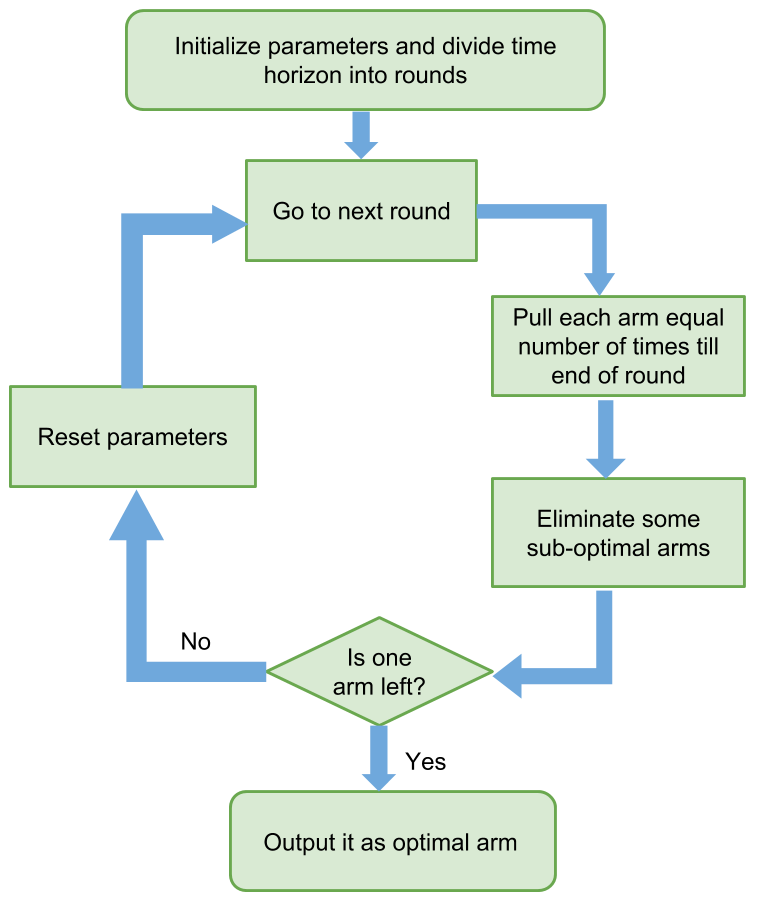
\includegraphics[scale=0.45]{Chapter2/img/Ucb-Imp.png}
\caption{Flowchart of UCB-Improved}
\label{fig:ucbimp}
\end{figure}
    
    UCB-Improved incurs a gap-dependent regret bound of $O\left(\frac{K\log (T\Delta^{2})}{\Delta}\right)$, which is better than that of UCB1. On the other hand, the worst case gap-independent regret bound of UCB-Improved is $O\left(\sqrt{KT\log K}\right)$. 
    
    Empirically, UCB-Improved is out-performed by UCB1 in almost all environments. This stems from the fact that UCB-Improved is pulling all arms equal number of times in each round and hence spends a significant number of pulls in initial exploration as opposed to UCB1 thereby incurring higher regret.
        
    
\subsubsection{MOSS Algorithm}    

\begin{algorithm}[!th]
\caption{MOSS}
\label{alg:moss}
\begin{algorithmic}[1]
\State \textbf{Input:} Time horizon $T$, $K$ number of arms with unknown parameters of reward distribution
\State Pull each arm once
 \For{$t=K+1,..., T$}
\State Pull the arm such that $\argmax_{i\in \A}\bigg\lbrace\hat{r}_{i} + \sqrt{\dfrac{\max\lbrace 0,\log(\frac{T}{K z_i})\rbrace}{z_i}}\bigg\rbrace$
\State $t:=t+1 $
 \EndFor
\end{algorithmic}
\end{algorithm}
    
    In the later work of \citet{audibert2009minimax}, the authors propose the MOSS algorithm which stands for Minimax Optimal Strategy in the Stochastic case (see Algorithm \ref{alg:moss}). The confidence interval of MOSS is designed in such a way so as to divide the horizon $T$ proportionally between the number of arms $K$ and the number of pulls $z_i$ that each arm is pulled. As the sub-optimal arms are pulled more number of times their confidence interval decreases, indicating that they have been explored sufficiently, forcing MOSS to explore other arms and quickly converging on the optimal arm. Theoretically, \citet{audibert2009minimax}  showed that the worst case gap-independent regret bound of MOSS is $O\left( \sqrt{KT} \right)$ which improves upon UCB1 by a factor of order $\sqrt{\log T}$. However, the gap-dependent regret of MOSS is $O\left( \frac{K^{2}\log\left(T\Delta^{2}/K\right)}{\Delta}\right)$ and in certain regimes, this can be worse than even UCB1 (see \citet{audibert2009minimax,lattimore2015optimally}). 
    
\subsubsection{OCUCB Algorithm}   

\begin{algorithm}[!th]
\caption{OCUCB}
\label{alg:ocucb}
\begin{algorithmic}[1]
\State \textbf{Input:} Time horizon $T$, $K$ number of arms with unknown parameters of reward distribution, exploration parameter $\alpha$ and $\psi$
\State Pull each arm once
 \For{$t=K+1,..., T$}
\State Pull the arm such that $\argmax_{i\in \A}\bigg\lbrace\hat{r}_{i} + \sqrt{\dfrac{\alpha\log(\psi\frac{T}{t})}{z_i}}\bigg\rbrace$
\State $t:=t+1 $
 \EndFor
\end{algorithmic}
\end{algorithm}

Recently in \citet{lattimore2015optimally}, the authors proposed the Optimally Confident UCB (OCUCB) (see Algorithm \ref{alg:ocucb}) which incorporates the increasing timestep $t$ in the confidence interval along with the fixed horizon $T$ and exploration parameters $\psi$ and $\alpha$. The authors showed that the algorithm OCUCB achieves order-optimal gap-dependent regret bound of $O\left(\sum_{i=2}^{K}\frac{\log\left(T/H_i\right)}{\Delta_i}\right)$ where $H_i=\sum_{j=1}^{K}\min\left\lbrace \frac{1}{\Delta_i^2},\frac{1}{\Delta_j^2}\right\rbrace$, and a gap-independent regret bound of $O\left( \sqrt{KT}\right)$. This is the best known gap-dependent and gap-independent regret bounds in the stochastic MAB framework. However, unlike our proposed EUCBV algorithm (in Chapter \ref{chap:EUCBV}), OCUCB does not take into account the variance of the arms; as a result, empirically  we find  that our algorithm outperforms OCUCB in all the environments considered.



\subsubsection{UCB-Variance Algorithm}

\begin{algorithm}[!th]
\caption{UCBV}
\label{alg:ucbv}
\begin{algorithmic}[1]
\State \textbf{Input:} $K$ number of arms with unknown parameters of reward distribution
\State Pull each arm once
 \For{$t=K+1,..., T$}
\State Pull the arm such that $\max_{i\in A}\bigg\lbrace\hat{r}_{i} + \sqrt{\dfrac{2\hat{v}_i\log (t)}{z_i}} + \dfrac{3\log (t)}{2}\bigg\rbrace$
\State $t:=t+1 $
 \EndFor
\end{algorithmic}
\end{algorithm}


    In contrast to the above work, the UCB-Variance (UCBV) algorithm in \citet{audibert2009exploration} utilizes variance estimates to compute the confidence intervals for each arm. In UCBV (see Algorithm \ref{alg:ucbv}) the confidence interval term is given by $\sqrt{\dfrac{2\hat{v}_i\log (t)}{z_i}} + \dfrac{3\log (t)}{3}$ where $\hat{v}_i$ denotes the empirical variance of the arm $i$. Hence, the confidence interval makes sure that the arms whose variances are high are pulled more often to get a better estimates of their $\hat{r}_i$.
    
    UCBV has a gap-dependent regret bound of $O\left(\frac{K\sigma_{\max}^{2}\log T}{\Delta}\right)$, where $\sigma_{\max}^{2}$ denotes the maximum variance among all the arms $i\in \A$. Its gap-independent regret bound can be inferred to be same as that of UCB1 i.e $O \left(\sqrt{KT\log T}\right)$. Empirically, \citet{audibert2009exploration} showed that UCBV outperforms UCB1 in several scenarios. 


\subsection{Bayesian Approach}

\begin{algorithm}[!th]
\caption{Bernoulli Thompson Sampling}
\label{alg:ts}
\begin{algorithmic}
\State {\bf Input:} $K$ number of arms with unknown parameters of reward distribution
\State {\bf Initialization:} For each arm $i:=1$ to $K$ set $S_i =0$ and $F_i =0$
\State \For{$t=1,..,T$}
\State \For{$i=1,..,K$}
\State Sample $\theta_{i}(t)$ from the $Beta(S_i+1,F_i+1)$ distribution.
\EndFor
\State Play the arm $i(t):=\argmax_i\theta_i(t)$ and observe reward $X_{i,t}$.
\If{$X_{i,t}=1$}
$S_i (t) = S_i (t) + 1$
\Else{$F_i (t) = F_i (t) + 1$}
\EndIf
\EndFor
\end{algorithmic}
\end{algorithm}

    
    Another notable design principle which has recently gained a lot of popularity is the Thompson Sampling (TS) algorithm (\citep{thompson1933likelihood}, \citep{agrawal2011analysis})  and  Bayes-UCB (BU) algorithm \citep{kaufmann2012bayesian}. This TS is stated in Algorithm \ref{alg:ts}. The TS algorithm is initialized with a uniform prior and it maintains a posterior reward distribution for each arm; at each round, the algorithm samples values from these distributions and the arm corresponding to the highest sample value is chosen. Although TS is found to perform extremely well when the reward distributions are Bernoulli, it is established that with Gaussian priors the worst-case regret can be as bad as $\Omega \left( \sqrt{KT\log T}\right)$ \citep{lattimore2015optimally}. The BU algorithm is an extension of the TS algorithm that takes quartile deviations into consideration while choosing arms.

\subsection{Information Theoretic Approach}
    
    The final design principle we state is the information theoretic approach of DMED  \citep{honda2010asymptotically} and KLUCB \citep{garivier2011kl},\citep{cappe2013kullback} algorithms. The algorithm KLUCB uses Kullbeck-Leibler divergence to compute the upper confidence bound for the arms. KLUCB is stable for a short horizon and is known to reach the \citet{lai1985asymptotically} lower bound in the special case of Bernoulli distribution. However, \citet{garivier2011kl} showed that KLUCB, MOSS and UCB1 algorithms are empirically outperformed by UCBV in the exponential distribution as they do not take the variance of the arms into consideration.
    
\subsection{Discussion on The Various Confidence Intervals}

A comparative analysis of the confidence interval of the UCB algorithms is discussed in table \ref{tab:conf-comp}. 

\begin{table}[!ht]
\caption{Confidence interval of different algorithms}
\label{tab:conf-comp}
\begin{center}
\begin{tabular}{|p{5em}|p{10em}|p{4em}|p{12em}|}
\hline
Algorithm  &  Confidence interval & Horizon as input & Remarks \\
\hline
\hline
UCB1        & $\sqrt{\dfrac{2\log (t)}{z_i}}$ & No & Loose confidence interval leading to high regret upper bounds.\\%\midrule
\hline
\hline
UCBV        & $\sqrt{\dfrac{2\hat{v}_i\log (t)}{z_i}} + \dfrac{3\log (t)}{2}$ & No & Confidence interval uses variance estimation.\\
\hline
\hline
UCB-Imp 		& $\sqrt{\dfrac{\log{( T\epsilon_{m}^{2})}}{2 n_{m}}}$ & Yes & Same confidence interval for all arms in a particular round.\\%\midrule
\hline
\hline
MOSS	     	& $\sqrt{\dfrac{\max\lbrace 0,\log(\frac{T}{K z_i})\rbrace}{z_i}}$ & Yes & Confidence interval is based on dividing the horizon proportionally between $K$ arms and $z_i$ pulls for each arm.\\%\midrule
\hline
\hline
OCUCB     	& $\sqrt{\dfrac{2\log(\frac{2T}{t})}{z_i}}$ & Yes & Tightest confidence interval with exploration parameter $\alpha=2$, $\psi=2$ leading to order-optimal regret bounds.\\\midrule
\end{tabular}
\end{center}
%\vspace*{-2em}
\end{table} 